%\documentclass[14pt, notes]{beamer}
\documentclass[14pt]{beamer}

%\usepackage{pgfpages}
%\setbeameroption{show notes}
%\setbeameroption{show notes on second screen=right}

%encoding
\usepackage[utf8]{inputenc}

%language
\usepackage[english, russian]{babel}
\usepackage{amsmath}
\usepackage{bm}
\usepackage{graphicx}
\usepackage{hyperref}
\usepackage{setspace}
\usepackage{tikz}
\usepackage{adjustbox}
\usepackage{marvosym}
\usetikzlibrary{shapes,arrows,positioning}
\makeatletter
%\@ifundefined{verbatim@out}{\newwrite\verbatim@out}{}
\makeatother
\graphicspath{{images/}}%путь к рисункам

\usepackage{tikz}
\usetikzlibrary{shapes,arrows}

\tikzstyle{decision} = [diamond, draw, fill=blue!20, text width=4.5em, text badly centered, node distance=3cm, inner sep=0pt]
\tikzstyle{block} = [rectangle, draw, fill=blue!20, text width=11em, text centered, rounded corners, minimum height=2em]
\tikzstyle{line} = [draw, -latex    ]
\tikzstyle{cloud} = [draw, ellipse,fill=red!20, node distance=3cm, minimum height=2em]

\setbeamerfont{author in head/foot}{size=\small}
\setbeamerfont{title in head/foot}{size=\footnotesize}
\setbeamercovered{invisible}
\setbeamertemplate{navigation symbols}{}%remove navigation symbols

\title[Numerical modeling of artificial heart valve]{Numerical modeling of artificial heart valve}
\date{\today}
\author[Dolgov D.A.]{Dolgov D.A., Zakharov Y.N.}
\institute{Kemerovo State University \\
    \vspace{0.7cm}
    \vspace{0.7cm}
} 
\usetheme[numbers, totalnumbers, minimal, nologo]{Statmod}
% Привычный шрифт для математических формул
\usefonttheme[onlymath]{serif}

\definecolor{statmodblue}{RGB}{100,10,30}
\definecolor{statmodsand}{RGB}{244,215,103}

\begin{document}
\maketitle

%description of the problem
\begin{frame}
\frametitle{Introduction}
Artificial heart valves are an effective method to treat many cardiovascular diseases. They are one of the most sophisticated medical devices that are used in cardiac surgery because of their design features. There are many requirements to the functioning of the artificial heart valves - an ideal valve replacement should produce a low flow resistance, yield a small regurgitant volume, minimise turbulence, etc.
\end{frame}

% valves placement
\begin{frame}
\frametitle{Arrangement of the valves}
    \begin{center}
        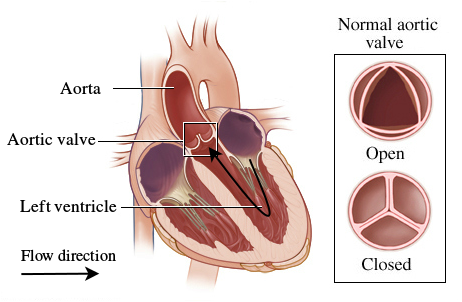
\includegraphics[width=8.5cm]{aorta_scheme.png}
    \end{center}
\end{frame}

\begin{frame}
\frametitle{Research overview}
    There are many researches, in which valves are of primary interest, while ignoring the fluid-structure interaction.
    \par
    {\tiny
        \begin{itemize}
            \item[\MVRightarrow] Bockeria L. A., Skopin I. I., Sazonenkov M. A., Tumaev E. N. Stress in valve leaflets and bioprosthesis in mitral position. Influence of fibrous ring on leaflet stress. // Clinical physiology of blood circulation, 2008, №2
            \item[\MVRightarrow] Kunzelman K.S., Reimink M.S. et al  Annular dilatation increases stress in the mitral valve and delays coaptation: a finite element computer model. (1997) Cardiovasc Surg 5(4):427–434
            \item[\MVRightarrow] Weinberg E. Dynamic simulation of heart mitral valve with transversely isotropic material model. Massachusetts Institute of Technology (2005)
            \item[\MVRightarrow] Kim H.S. Nonlinear multi-scale anisotropic material and structural models for prosthetic and native aortic heart valves. Georgia Institute of Technology (2009)
        \end{itemize}
    }
\end{frame}

\begin{frame}
\frametitle{Research overview}
    Most of the researches, which considering full fluid-structure interaction,
    are related to the immersed boundary method. But in the existing papers the fluid flow
    with admixtures is covered not enough.
    \par
    {\tiny
        \begin{itemize}
            \item[\MVRightarrow] Peskin, Charles S. "Numerical analysis of blood flow in the heart." Journal of computational physics 25.3 (1977): 220-252.
            \item[\MVRightarrow] Luo, X. Y., et al. "Effect of bending rigidity in a dynamic model of a polyurethane prosthetic mitral valve." Biomechanics and modeling in mechanobiology 11.6 (2012): 815-827.
            \item[\MVRightarrow] Flamini, Vittoria, Abe DeAnda, and Boyce E. Griffith. "Immersed boundary-finite element model of fluid-structure interaction in the aortic root." (2015).
        \end{itemize}
    }
\end{frame}

% valve tissue structure
\begin{frame}
\frametitle{Scheme of valve tissue structure}
    \begin{center}
        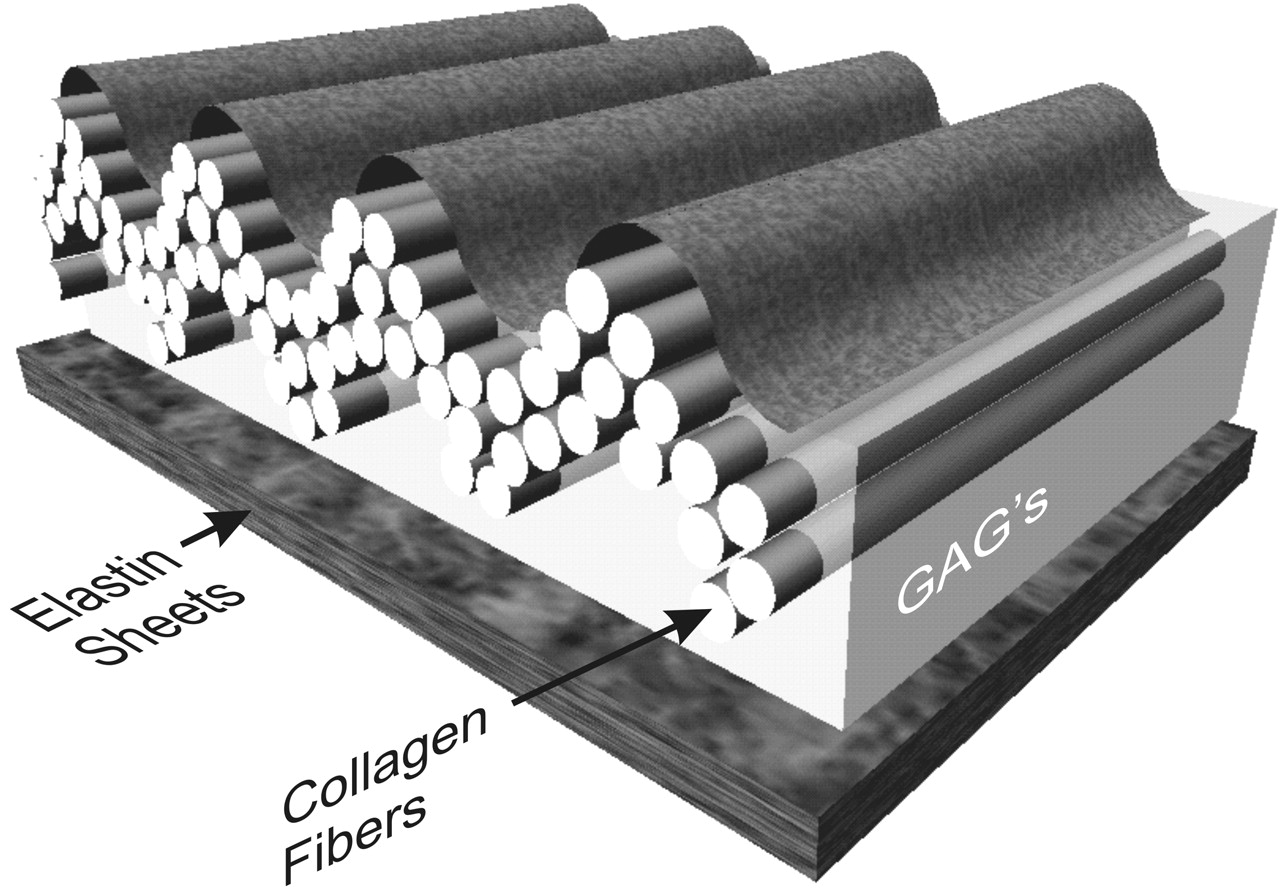
\includegraphics[width=8.5cm]{valve_tissue_structure.jpg}
    \end{center}

    \begin{spacing}{0.5}
        \mbox{\scriptsize
            Vesely, Ivan. "Heart valve tissue engineering." Circulation research 97.8 (2005): 743-755.
        }
    \end{spacing}

\end{frame}

% blood structure scheme
\begin{frame}
\frametitle{Scheme of blood structure}
    \begin{center}
        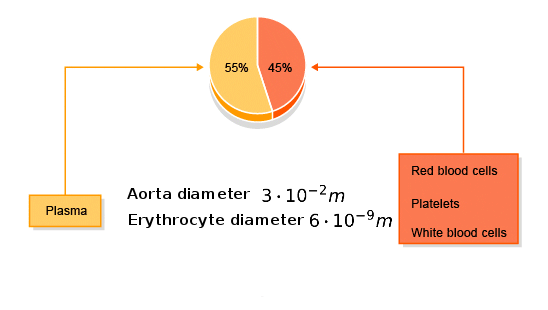
\includegraphics[width=8.5cm]{blood_scheme3.png}
    \end{center}
\end{frame}

\begin{frame}
\frametitle{Example of artificial heart valve}
    \begin{center}
        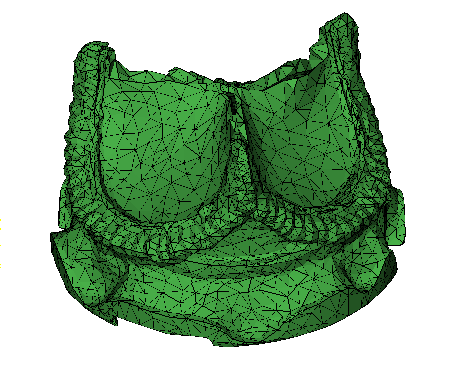
\includegraphics[width=6cm]{real_valve_3_1.png}
        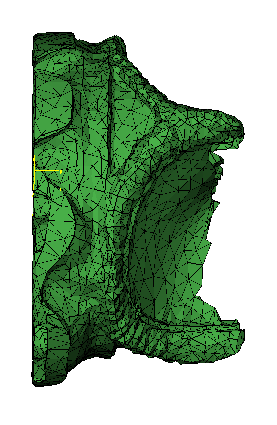
\includegraphics[width=3cm]{real_valve2_1.png}
    \end{center}
\end{frame}

\begin{frame}
\frametitle{Model description}
We will consider the problem of blood flow inside large vessels with flexible walls and valve.
Blood consists of plasma and formed elements. Valve leaflets are deformed under the fluid pressure.
We model the blood as a viscous incompressible inhomogeneous two component fluid with variable viscosity,
and vessel wall and valve leaflets as a fluid impermeable surface with specified stiffness.
\end{frame}

%description of the problem: schema
\begin{frame}
\frametitle{Model description}
    \begin{center}
        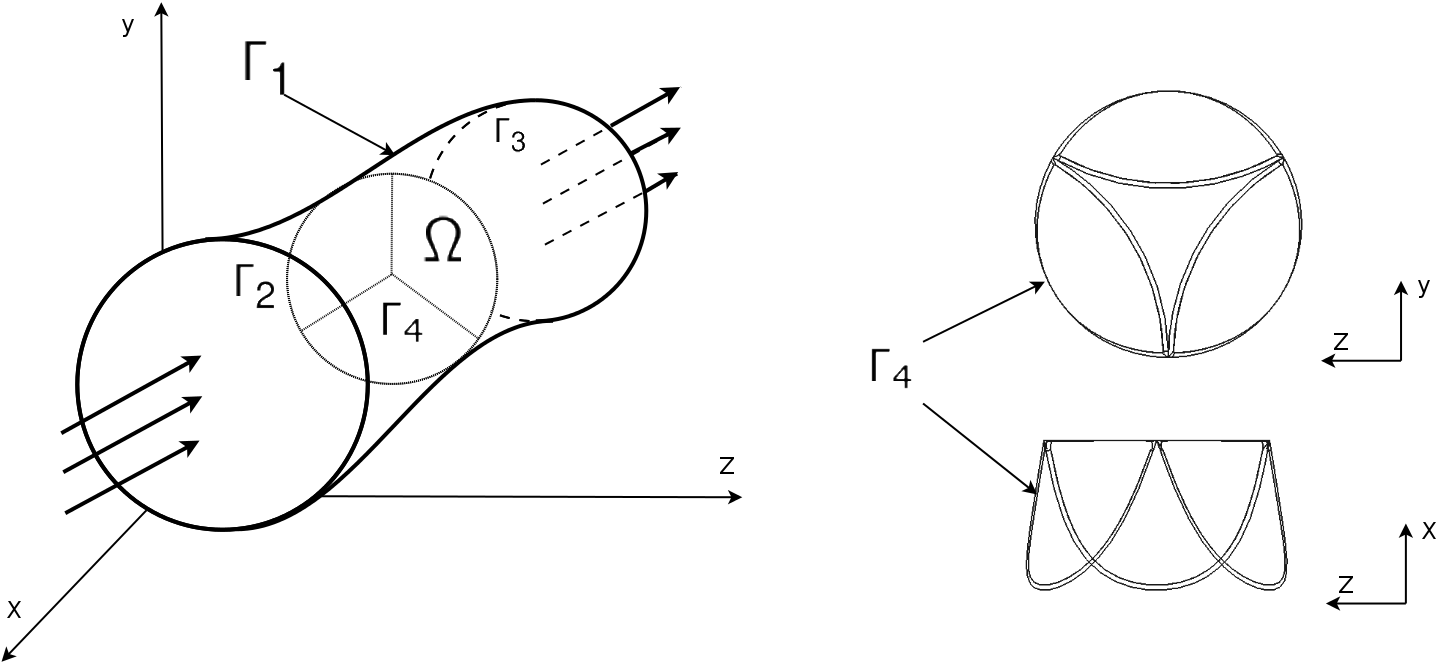
\includegraphics[width=8.5cm]{area_3d.png}
    \end{center}
\end{frame}

% navier stokes equations
\begin{frame}
\frametitle{Fluid flow}
Navier-Stokes system of equations:
\begin{gather}
    \label{eq:motion}
    \frac{\partial u}{\partial t} + (u \cdot \nabla) u = - \frac{1}{\rho} \nabla p + \nabla \cdot \sigma + f\\
    \label{eq:continuity}
    \frac{\partial \rho}{\partial t} + \nabla \cdot (\rho u) = 0 
\end{gather}
where $\sigma = \mu (\nabla u + (\nabla u)^{T})$, $\bar{x} = (x, y, z) \in \Omega$ with the initial and boundary conditions
\begin{gather*}
    u(\bar{x}, t_0) = u_0;\ \frac{\partial u}{\partial n}|_{\Gamma_2, \Gamma_3} = 0\\
    p|_{\Gamma_2} = p_{in};\ p|_{\Gamma_3} = p_{out} \\
\end{gather*}

\end{frame}

% concentration
\begin{frame}
\frametitle{Concentration}
An equation for the concentration of admixture in the fluid:
\begin{gather}
    \label{eq:concentration}
    \frac{\partial c}{\partial t} + u \cdot \nabla c = 0
\end{gather}
with the initial and boundary conditions
\begin{gather*}
    c(\bar{x}, 0) = c_0(\bar{x})\\
    c(\bar{x}, t)|_{\Gamma_2} = c_s(\bar{x}, t)
\end{gather*}

\end{frame}

% concentration: dependencies
\begin{frame}
\frametitle{Concentration}
Density and viscosity are depend from concentration:
\begin{gather}
    \label{eq:concentration_viscosity}
    \mu = c (\mu_2 - \mu_1) + \mu_1\\
    \label{eq:concentration_density}
    \rho = c (\rho_2 - \rho_1) + \rho_1
\end{gather}

where $\mu_1, \mu_2, \rho_1, \rho_2$ - viscosity and density of both components.
\end{frame}

% boundary
\begin{frame}
\frametitle{Deformation resistance}
Motion of the vessel walls and valve leaflets is defined by the forces, which return them to the original position.
\begin{gather}
    \label{eq:strain_energy}
    F =  \frac{\partial}{\partial s}(T \tau) + \frac{\partial^2}{\partial s^2} \Big( E \cdot I \frac{\partial^2}{\partial s^2} X \Big)
\end{gather}
\begin{gather}
    \label{eq:define_boundary_force}
    F = k \cdot \|X - X_0\|
\end{gather}
\end{frame}

% solve method 
\begin{frame}
\frametitle{Solution method}
We determine the fluid flow and the valve leaflets on the separate grids
\begin{itemize}
    \item[\MVRightarrow] $\Omega_h = \Omega_h(x, y, z)$ - uniform staggered grid for fluid.
    \item[\MVRightarrow] $\Gamma_h = \Gamma_h(q, r, s, t)$ - grid, related to the valve leavlets with Lagrangian coordinate system.
\end{itemize}

\end{frame}

% solve method: diagram
\begin{frame}
\frametitle{Solution method}
    \begin{center}
        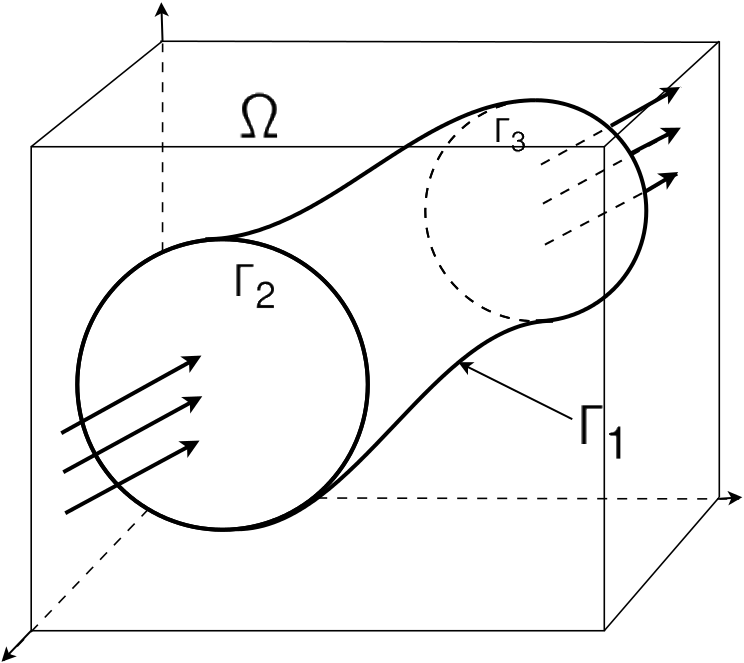
\includegraphics[width=8.5cm]{area_ibm_3d.png}
    \end{center}
\end{frame}

% solve method: diagram
\begin{frame}[fragile]
\frametitle{Algorithm}
    \begin{adjustbox}{max totalsize={1.0\textwidth}{.7\textheight},center}
        \begin{tikzpicture}[node distance = 2.5cm, auto]
            \node[block]                           (init){
                $u_0$, $p_0$, $\rho_0$, $\nu_0$
            };

            \node[block, fill=none, minimum height=25em, text width=14em]          (fluid) at (6.8, -5){
                $\Omega$
            };
            \node[block, right=1cm of init]            (body_forces_initial){
                body forces $f_{ijk} = 0$
            };
            \path[line] (init) --                  (body_forces_initial);

            \node[block, below of=body_forces_initial]            (navier_stokes){
                Navier-Stokes equations
            };
            \path[line] (body_forces_initial) --                  (navier_stokes);

            \node[block, below of=navier_stokes]   (concentration){
                concentration $c_{n+1}$
            };
            \path[line] (navier_stokes) --         (concentration);

            \node[block, below of=concentration]   (viscosity_density){
                $\mu_{n+1}$, $\rho_{n+1}$ recalculation
            };
            \path[line] (concentration) --         (viscosity_density);

            \node[block, below of=viscosity_density]   (new_flow){
                $u_{n+1}$, $p_{n+1}$, $\rho_{n+1}$, $\mu_{n+1}$
            };
            \path[line] (viscosity_density) --     (new_flow);

            \node[block, fill=none, minimum height=25em, text width=14em]          (fluid) at (14.8, -5){
                $\Gamma$
            };
            \node[block, right= of new_flow, anchor=west](boundary_velocity){
                new boundary velocity, $U_n$
            };
            \path[line] (new_flow) --         (boundary_velocity);

            \node[block, right=of viscosity_density, anchor=west](deformation){
                new boundary shape $X_{n+1}(X_{n}, U_{n}, t)$
            };
            \path[line] (boundary_velocity) --         (deformation);

            \node[block, right=of concentration, anchor=west](boundary_forces){
                deformation resistance $F_{n}(X_{n+1}, X_{n})$
            };
            \path[line] (deformation) --         (boundary_forces);

            \node[block, right=of navier_stokes, anchor=west](body_forces){
                new body forces distribution $f_{ijk}$
            };
            \path[line] (boundary_forces) --         (body_forces);
            \path[line] (body_forces) --         (body_forces_initial);
        \end{tikzpicture}
    \end{adjustbox}
\end{frame}

% solve method:split scheme
\begin{frame}
\frametitle{Solution algorithm: flow}
Splitting schemes due to physical factors:
\begin{gather}
    \label{eq:split_first}
    \frac{u^* - u^n}{\triangle t} = - (u^n \cdot \nabla) u^n + \frac{1}{\rho} \nabla \sigma + f\\
    \label{eq:split_second}
    \rho \triangle p^{n+1} - (\nabla p \cdot \nabla p^{n+1}) = \frac{\rho^2 \nabla u^*}{\triangle t}\\
    \label{eq:split_third}
    \frac{u^{n+1} - u^*}{\triangle t} = - \frac{1}{\rho} \nabla p^{n+1}
\end{gather}
where $\nabla \sigma (u^n, \mu) = \mu \triangle u^n + (\nabla \mu \cdot \nabla) u^n + (\nabla \mu \cdot J_{u^n}) $
\end{frame}


% solve method: boundary forces
\begin{frame}
\frametitle{Solution algorithm: valve}
\begin{gather}
    \label{eq:strain_energy}
    F_{n} =  \frac{\partial}{\partial s}(T_{n} \tau_{n}) + \frac{\partial^2}{\partial s^2} \Big( E \cdot I \frac{\partial^2}{\partial s^2} X_{n} \Big)
\end{gather}
\end{frame}


% solve method:immersed boundary
\begin{frame}
\frametitle{Fluid-structure interaction}
Interaction between valve leaflets and fluid flow:
\begin{gather}
    \label{eq:ibm_velocity}
    \frac{\partial X}{\partial t} = \int_{\Omega_h} u \cdot \delta (\bar{x} - X)\; dx\; dy\; dz \\
    \label{eq:ibm_force}
    f = \int_{\Gamma_h} F \cdot \delta (\bar{x} - X)\; dq\; dr\; ds\\
    \label{eq:no_slip}
    \frac{\partial X}{\partial t} (q, r, s, t) = u(X(q, r, s, t), t)
\end{gather}
\end{frame}

% solve method:ibm scheme
\begin{frame}
\frametitle{Fluid-structure interaction}
Interpolation of the flow velocity on the immersed boundary, and new body forces distribution:
\begin{gather}
    \label{eq:interpolation}
    U_n = \sum_{ijk}u_{ijk} \cdot D(x_{ijk} - x_n) h_{ijk}^3 \\
    \label{eq:spreading}
    f_{ijk} = \sum_n F_n \cdot D(x_{ijk} - x_n) h^2_n
\end{gather}

$D(x_n)$ corresponds to $\delta(x - x_k)$.
\end{frame}

% totals and examples
\begin{frame}
\frametitle{Results}
    \begin{center}
        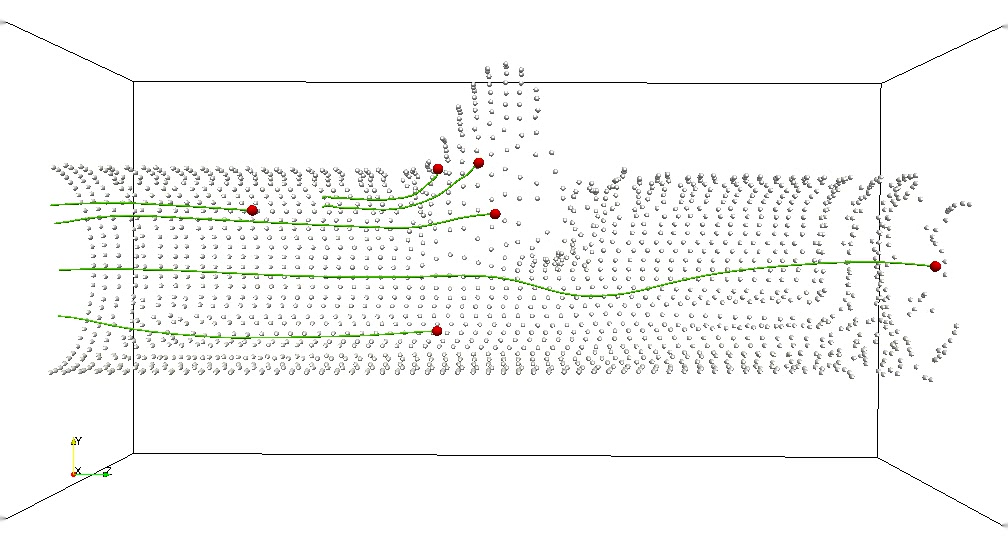
\includegraphics[width=9cm]{cylinder2_avi.png}
    \end{center}

\begin{itemize}
    \item[\MVRightarrow] \href{run:video/cylinder2.avi}{Vessel wall deformation}
\end{itemize}
\end{frame}

% totals and examples
\begin{frame}
\frametitle{Results}
    \begin{center}
        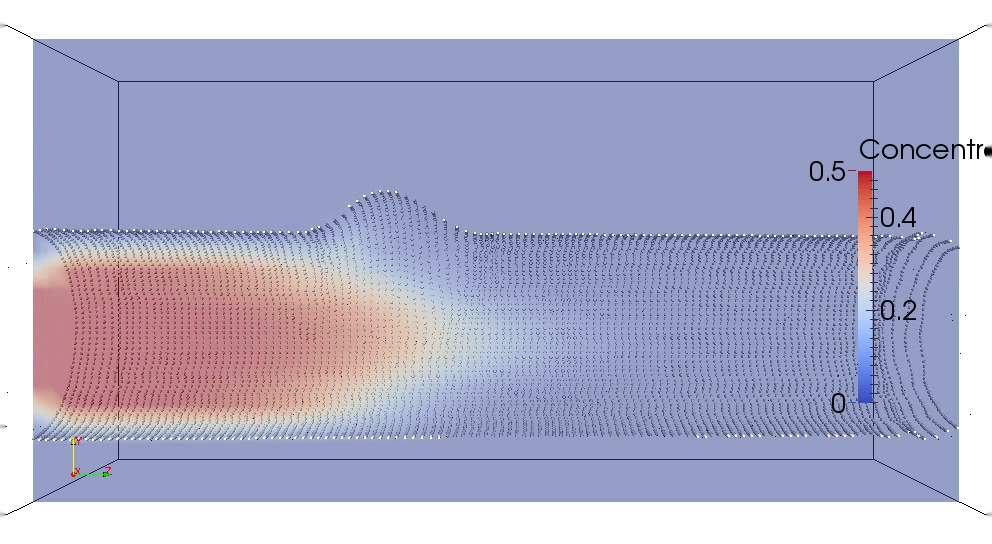
\includegraphics[width=5cm]{source_in_vessel_avi.png}
        \vspace{0.40mm}
        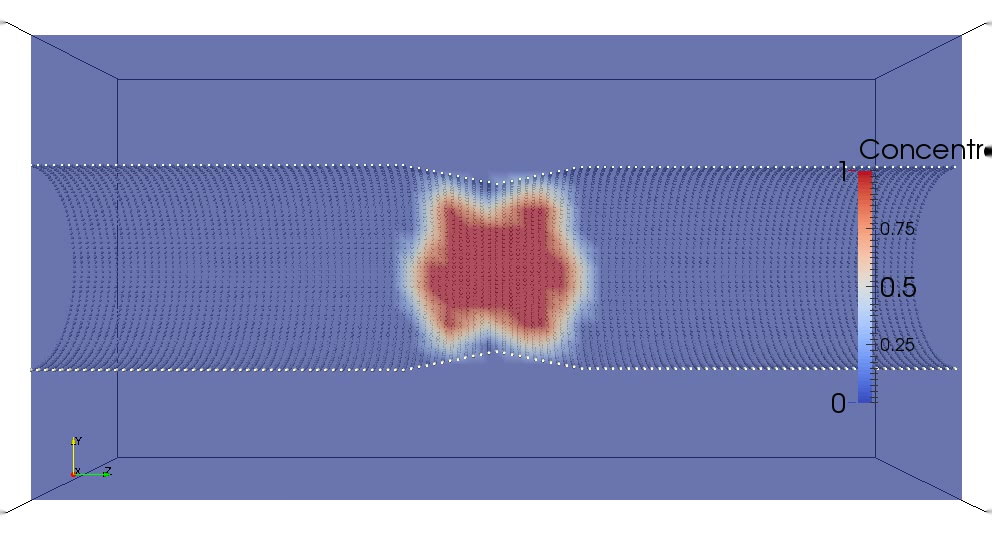
\includegraphics[width=5cm]{thrombus_in_vessel_avi.png}
    \end{center}

\begin{itemize}
    \item[\MVRightarrow] \href{run:video/source_in_vessel.avi}{Admixture propagation}
    \item[\MVRightarrow] \href{run:video/thrombus_in_vessel.avi}{"Thrombus"}
\end{itemize}
\end{frame}

\begin{frame}
\frametitle{Results}
    \begin{center}
        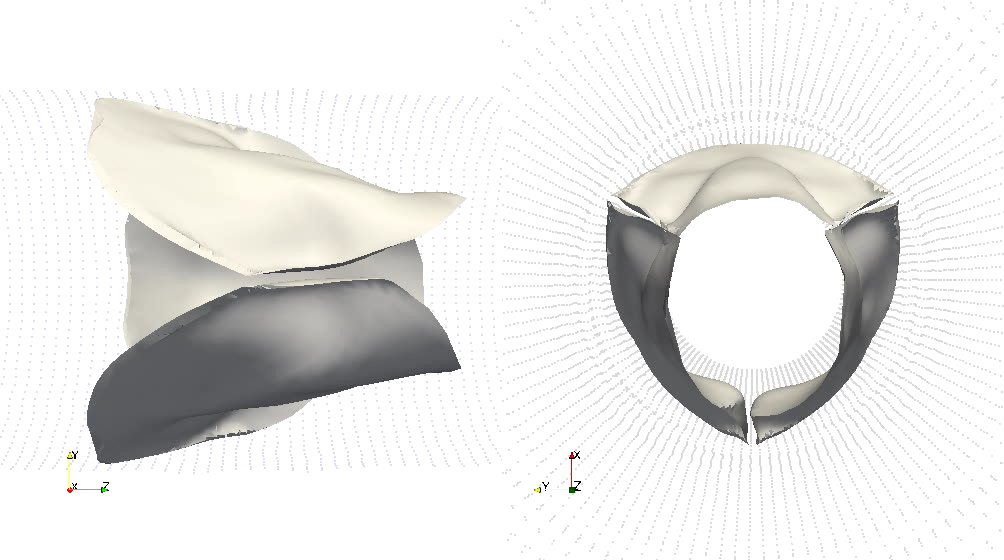
\includegraphics[width=9cm]{valve_delaunay3_2.png}
    \end{center}

\begin{itemize}
    \item[\MVRightarrow] \href{run:video/valve_delaunay3.avi}{Motion of the valve leaflets}
\end{itemize}
\end{frame}

\begin{frame}
\frametitle{Results}
    \begin{center}
        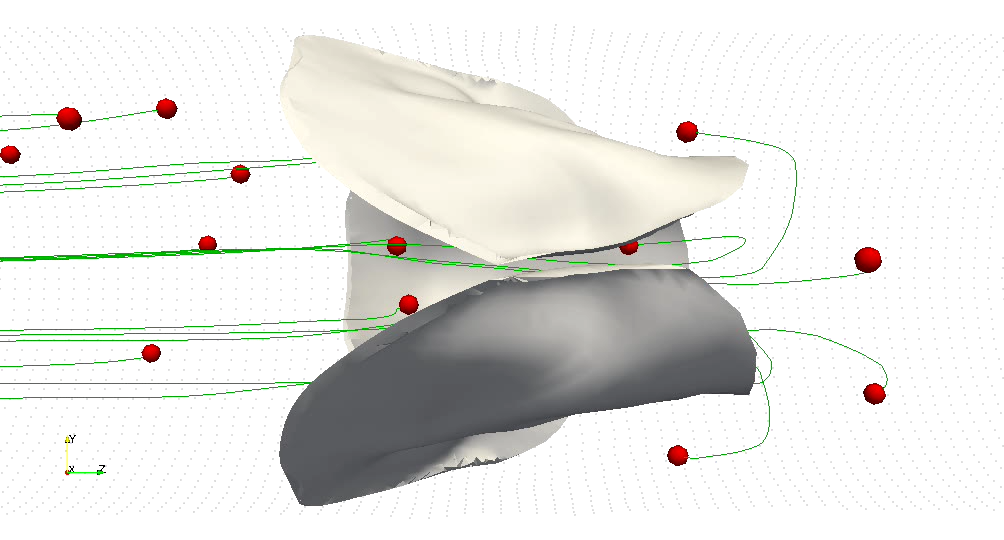
\includegraphics[width=9cm]{valve_markers3.png}
    \end{center}

\begin{itemize}
    \item[\MVRightarrow] \href{run:video/valve_markers_better.avi}{Tracks of particles inside the valve}
\end{itemize}
\end{frame}

%\begin{frame}
%\frametitle{Примеры}
    %\begin{center}
        %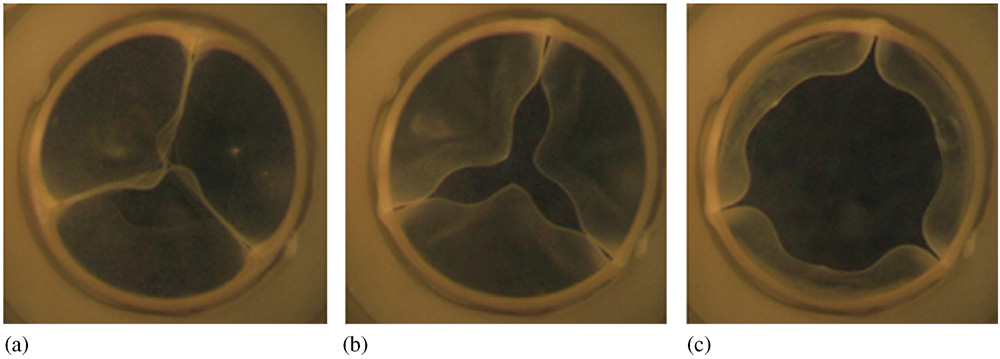
\includegraphics[width=11cm]{aortic_valves.jpg}
    %\end{center}

%\begin{spacing}{0.5}
%{\scriptsize
    %Watton PN, Luo XY et al (2007) Dynamic modelling of prosthetic
    %chorded mitral valves using the immersed boundary method.
    %J Biomech 40(3):613–626 Watton PN, Luo XY et al (2008) Effect of ventricle motion on the
%}
%\end{spacing}

%\end{frame}

\begin{frame}
\frametitle{Fluid flow rate}
    \begin{center}
        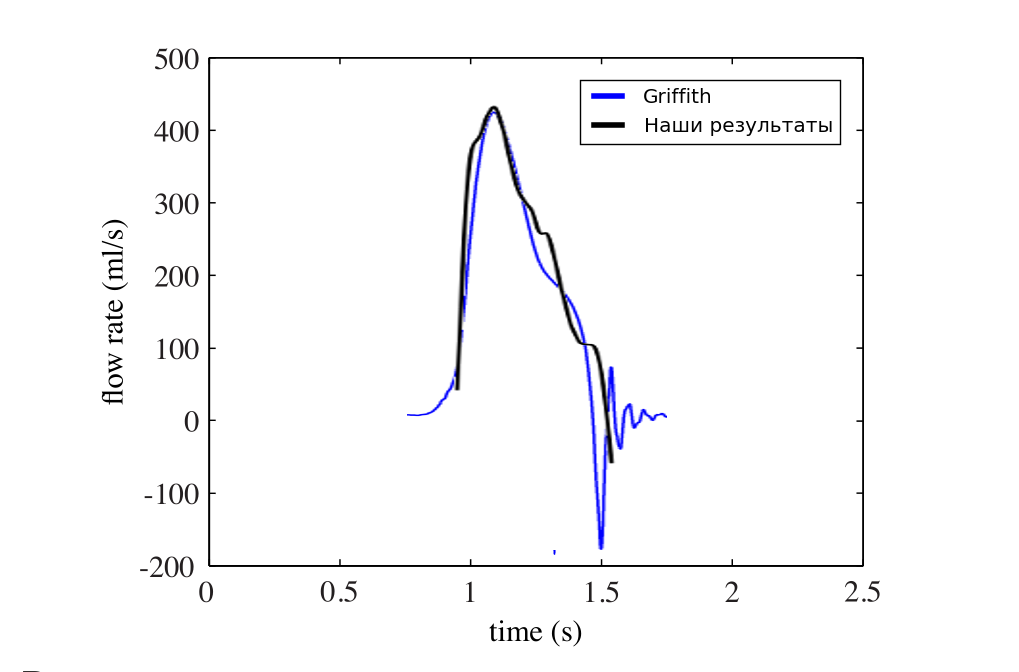
\includegraphics[width=10cm]{flow_rate_comparison_with_legend.png}
    \end{center}

    \begin{adjustbox}{max totalsize={1.0\textwidth}{.7\textheight},center}
        {\scriptsize
            International Journal for Numerical Methods in Biomedical Engineering 28.3 (2012): 317-345.
            %"Immersed boundary model of aortic heart valve dynamics with physiological driving and loading conditions." International Journal for Numerical Methods in Biomedical Engineering 28.3 (2012): 317-345.
        }
    \end{adjustbox}
\end{frame}
\end{document}
